\newpage
\section{Introduction}
\todo[inline]{/{This section shall introduce the reader to the subject addressed by the report. It should include i) a brief explanation of how a brake-by-wire system works and its main advantages and drawbacks compared to existing brake systems, and ii) a description of the purpose of the report, i.e., a formulation of the problem to which the report provides an answer. The last paragraph should consist of a “roadmap” of the report.}/}

The purpose of this laboratory assignment is to gain understanding about how dependability modeling can be applied to evaluate fault-tolerant systems. In this report, two different design solutions for a brake-by-wire systems is evaluated.
 
In a brake-by-wire system, the conventional hydraulic is replaced by an electronic system. The advantage to use a electronic system instead of the conventional is lower weight, lower cost, and simpler integration with other electronic systems already in use, such as active safety systems and stability control. 


The model used for a brake-by-wire system is shown in \figref{bbwsys} and comprises of a central unit (CU) that receives sensor data about the car's movement and anticipated movement, four wheel units (WU) that measures and controls the rotation of a wheel, and serial buses (SB1 and SB2) for communication. To ensure fault tolerant behavior, the CU and WU are implemented using redundant components when found necessary, and the communication buses are duplicated. 

Individual brake commands is derived for the wheels with respect to the received sensor data and these computations can either be performed in the CU or in the WUs. The first architecture is called the distributed architecture, where the computations are performed in the WUs. The second architecture is called the centralized architecture, where the computations are performed in the CU.

The report are organized as follows. In \secref{S2}, the two design solutions are presented. In \secref{S3} is the dependability models used in the report explained. In \secref{S4} are the results presented. In \secref{S5}, the results are discussed and the report is conluded in \secref{S6}.

\begin{figure}[h!]
  \centering
  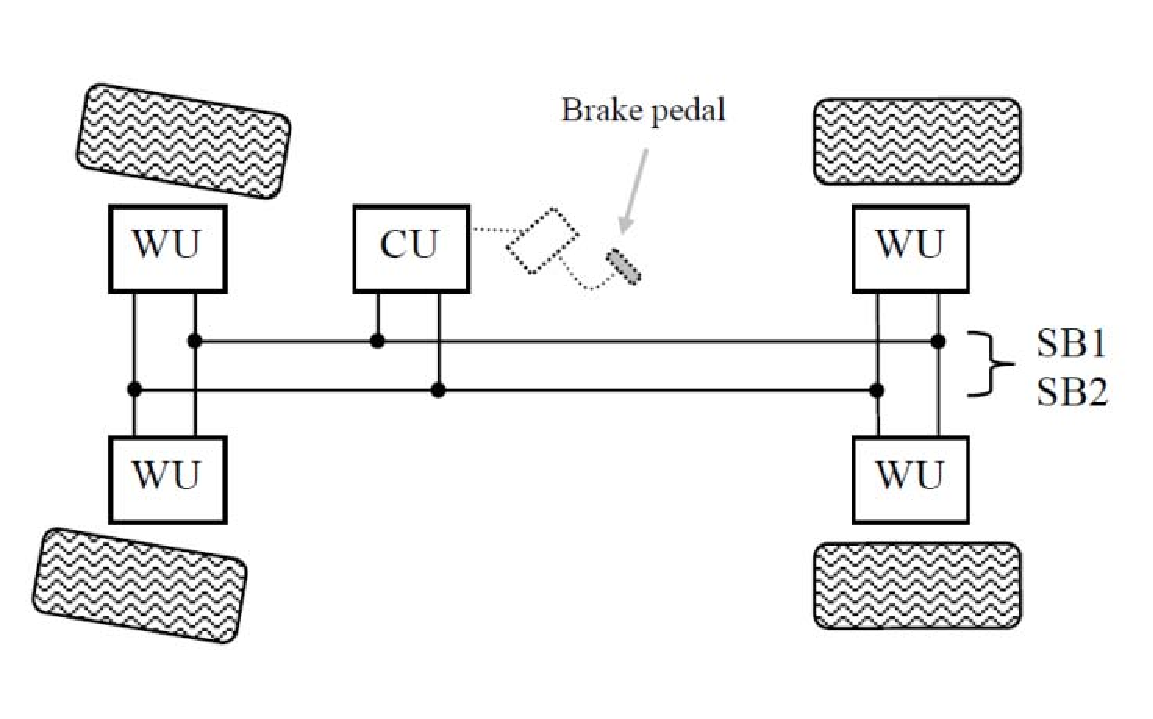
\includegraphics[scale=.5]{Fig1.pdf}
  \caption{Brake-by-wire system}
  \label{bbwsys}
\end{figure}